\section{Introduction}

As distributed data-parallel computing matures, throughput-sensitive batch processing systems \cite{mapreduce, dryad, graphlab, tez} are increasingly being complemented by latency-sensitive interactive analytics \cite{spark, blinkdb, presto} and online stream processing systems \cite{spark-streaming, trident, millwheel, naiad, flink}. 
To enable data sharing and seamless transition between these models, all these applications coexist on shared clusters \cite{google-dataflow-cloud, databricks-cloud, bdas, mesos, yarn, kubernetes, dc-computer}.
Naturally, both systems and networking communities have focused on resource sharing in these clusters \cite{mesos, yarn, apollo, hadoop-capacity-scheduler, varys, oktopus}. 

Today's schedulers are multi-resource \cite{drf, tetris, multiresource-mungchiang, orchestra, pacman}, DAG-aware \cite{aalo, tetris, spark}, and allow a variety of constraints \cite{late, quincy, mantri, choosy, delay-scheduling}. 
Given all these inputs, they optimize for objectives such as fairness \cite{drf, jaffe-maxmin, drfq, hdrf}, performance \cite{sjf}, efficiency \cite{tetris}, or different combinations of the three \cite{carbyne, graphene}.
% Fairness is often the primary objective in shared clusters \cite{apollo, late, hadoop-capacity-scheduler, tetris, drf, jaffe-maxmin, hdrf, carbyne, hug}, because it ensures performance isolation between multiple entities.
% A fair scheduler divides multiple resources based on the number of jobs (or the number of job queues) present in the cluster.\footnote{If jobs have different weights, one can use weighted fairness.}
However, all existing schedulers have one thing in common: \emph{they force the same performance goal on all jobs}.

Even though batch, interactive, and streaming computation models all care about performance, their notions of performance are different.
For instance, the average completion time can sufficiently capture the performance of a throughout-sensitive batch-job queue (\batchq) \cite{tetris, carbyne, mantri, late}.
However, interactive sessions and streaming applications form latency-sensitive queues (\burstq): each \burstq is a sequence of small jobs following an ON-OFF pattern. 
For these jobs \cite{spark-streaming, spark, splunk-analysis, presto}, individual completion times or latencies are far more important than the average completion time or the throughput of the \burstq. 

Indeed, existing ``fair'' schedulers are inherently unfair to \burstq jobs: when \burstq jobs are present (ON state), they must share the resources equally with \batchq jobs, but when they are absent (OFF state), batch jobs get all the resources. 
The fact that \burstq jobs are not using any resources during their OFF periods is completely ignored.
In the long run, {\batchq}s receive more resources than their fair shares because today's schedulers make \emph{instantaneous} decisions (\S\ref{sec:motivation}).

One may assume that assigning higher priorities to {\burstq} jobs (Strict Priority, or SP~\cite{strict_priority}) would resolve this. 
Although simple and attractive, prioritization cannot address this challenge because it incentivizes {\burstq}s to submit arbitrarily large jobs to starve {\batchq}s. 
Consequently, the performance-isolation tradeoff requires a careful consideration. 

Additionally, how one reasons about system utilization becomes more complicated in the presence of both {\burstq}s and {\batchq}s. 
While it is relatively easy to fill the cluster with many batch jobs to achieve high utilization, {\burstq}s often have higher value and are harder to accommodate with resource guarantees. 
Compared to a simple solution that rejects most of {\burstq}s and/or serves them with best efforts, system operators are likely to prefer to maximize the {\burstq}s served with resource guarantees, which leads to more predictable performance. %We call the resources allocated to {\burstq}s with resource guarantees {\burstq} utilization.

Therefore, we ponder a fundamental question: \emph{can we enable latency-sensitive {\burstq}s and throughput-sensitive {\batchq}s to coexist, where {\burstq}s are permitted short-term resource bursts while ensuring long-term fairness between the two, as well as maximizing {\burstq}s served with resource guarantees?}

The need to separate throughput- and latency-sensitive job queues in big data clusters is akin to the classic networking problem of supporting throughput-sensitive flows and latency-sensitive realtime communication on network access links \cite{cbq, intserv-hierarchy, hfsc, cruz-sc}.
The key difference between the two is the multi-resource nature of cluster scheduling and challenges arising from it. 
We aim for a solution that can be applied to multi-resource clusters.

%\todo{five properties, but some are missing below.}
In this paper, we first explore opportunities and challenges in achieving four desired properties in this context (\S\ref{sec:motivation}): (i) allowing {\burstq}s to enjoy short-term high resource usage during their ON periods to minimize \emph{individual} job response times; (ii) maintaining the same \emph{long-term} fairness as existing multi-resource fair allocation policies by preventing arbitrarily large bursts; (iii) maximizing system utilization and {\burstq}s served with resource guarantees; %\new{(iv) It is better off sharing than using static sharing}. 
and (iv) the policy needs to be strategyproof because otherwise {\burstq}s may lie about their demands to gain more resources. 

The key opportunity lies in the observation that {\batchq}s do not care about allocated resources in the short term, as long as the long-term averaged resource share remains the same. 
This temporal flexibility allows us to accommodate bursts of {\burstq}s without hurting {\batchq}s. 
% Significant performance improvement potential is demonstrated by an example in Figure~\ref{fig:motiv_ex}.
However, there are several challenges to achieve these desired properties (\S\ref{sec:motivation}). There is a fundamental tradeoff between ``hard'' resource guarantee to {\burstq}s and instantaneous isolation protection for {\batchq}s. 
In addition, naive admission control may result in very few {\burstq}s admitted with resource guarantees, leading to suboptimal performance for {\burstq}s even with a high system utilization. %\nhattan{needs to explain the properties here.}

\begin{figure}[!t]
  \centering
  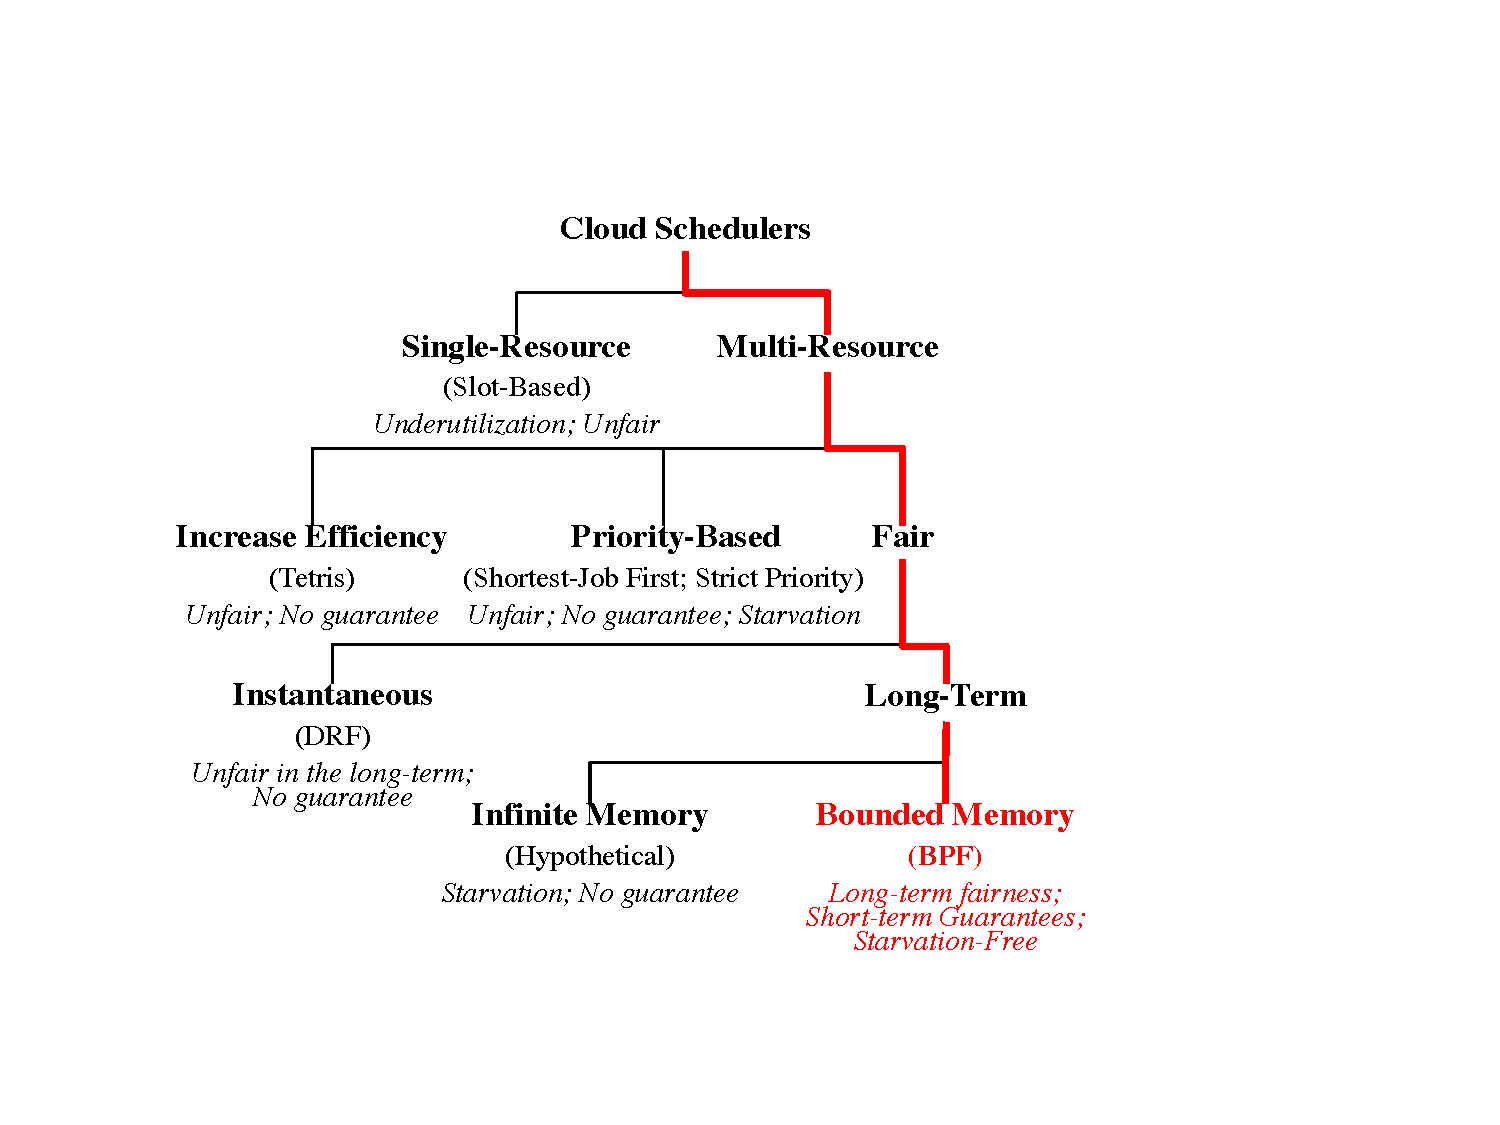
\includegraphics[width=\columnwidth]{fig/Design-Space.pdf}%
  \caption{Cluster scheduling design space.}%
  \label{fig:design-space}
\end{figure}

\subsection*{Contributions}

\paragraph{Algorithm development.}
%We present {\name} to find a balance between batch and bursty queues without unfairly tipping the balance toward either direction (\S\ref{sec:approach}). 
We present {\name} in Section~\ref{sec:approach} to find a balance between the potentially conflicting properties. 
Given the performance-isolation tradeoff, {\name} takes long-term fairness as the hard requirement as otherwise {\batchq}s may starve, which is not acceptable. 
Under the isolation requirement, {\name} tries to optimize the other two metrics: individual completion time of {\burstq}s and number of {\burstq}s admitted with resource guarantees. 

In {\name}, an {\burstq} reports on its arrival the inter-arrival time and maximum allowed processing time (and therefore the deadlines), as well as the amount and duration of (multiple typed) resources requested. An upper limit on the cycle length is set to respect the fair share of {\batchq}s in a timely manner. 
{\name} then decides whether to admit the {\burstq} by checking the safety condition, i.e., admitting this {\burstq} does not invalidate any prior resource guarantees committed. Then, if its total requested resources exceed its long-term fair share, the {\burstq} is admitted and provided only with its long-term fair share. Otherwise, the {\burstq} is admitted with resource guarantees. \name provides both hard and soft guarantees.   
Intuitively, if there are enough available resources for every burst of the {\burstq}, it is admitted with hard guarantee, i.e., the system guarantees to provide the requested amount of resources during each requested interval accordingly. 
Otherwise, the {\burstq} is admitted with soft guarantee, i.e., the requested amount of resources are provided as long as there is no conflict with {\burstq}s with hard guarantee. 

Having the queue with soft guarantee is crucial to minimize the individual completion time of {\burstq}s. 
While {\burstq}s with hard guarantee are provided with performance comparable to that under SP, {\burstq}s with soft guarantee can still have better performance compared to that under existing fair allocation policies. 
%Compared to simply rejecting {\burstq}s with soft guarantee, overall good utilization increases. 

For long-term fairness and isolation, {\name} guarantees a fixed amount of resources to each admitted {\burstq} instead of extending unlimited resources by prioritization. 
If some {\burstq} increases their demand beyond its resource guarantee, that demand is only served when the system has unused resources without hurting the isolation for {\batchq}s and other {\burstq}s. 

The analysis of \name is in \S\ref{sec:properties-theorem}, where strategyproofness is proved in addition to the other properties. To the best of our knowledge, \name is the first multi-resource scheduler that can provide all the five properties. 

%\paragraph{Analysis of properties.} \new{We show that {\name} satisfy all the critical properties, i.e., long-term fairness (LF), burst guarantee (BG), sharing incentive (SI), and strategyproofness (SPF), and pareto efficiency (PE) (\S\ref{sec:properties-theorem}). The other comparable approaches like Strict Priority and the combination of DRF with BVT cannot achieve more than three of the five properties (\S\ref{sec:property-analysis}).}

\paragraph{Design and implementation.} We have implemented \name on Apache YARN \cite{yarn} (\S\ref{sec:impl}).
Any framework that runs on YARN can take advantage of \name.
The \name scheduler is implemented as a new scheduler in Resource Manager that runs on the master node.
The scheduling overheads for admitting queues or allocating resources are negligibly less than 1 ms for 20,000 queues.

\paragraph{Evaluation based on both testbed experiments and large-scale simulations.}
We deployed and evaluated \name on 40 bare-metal machines using the public benchmarks, i.e., BigBench (BB) \cite{bbench}, TPC-DS \cite{tpc-ds}, and TPC-H \cite{tpc-h}.
In deployments, \name significantly provides up to $5.38\times$ (totally 9 queues in a cluster) faster performance with smaller variation for \burstq jobs than DRF, while maintaining the fairness among the queues (\S\ref{sec:testbed}). 
In fact, the performance of \burstq jobs is close to that under SP. 
%In addition, \name provides smaller variations in completion times to \burstq jobs. %while DRF is negatively impacted by the workload demand.
%In fact, 
On the other hand, \name maintains the fairness among the queues and does not hurt the long-term averaged resources received by {\batchq}s.
\name protects the {\batchq} jobs up to $3.05\times$ compared to SP.
Furthermore, \name performs well even in the presence of moderate misestimations of task demands and without preemption allowed (\S\ref{sec:sensitivity_analysis}).

%We discuss related work in Section~\ref{sec:related}.

%\mosharaf{A list of three contributions? Problem formulation, Algorithm and its properties, and full system evaluation and thorough eval.}
